%\documentclass[a4paer]{article}
%\documentclass[12pt,onecolumn]{IEEEtran}
%\linespread{1.6}
%\documentclass[11pt,journal,comsoc]{IEEEtran}
\documentclass[journal]{IEEEtran}

\usepackage{amsmath}
%\usepackage{booktabs}

%\usepackage[cmintegrals]{newtxmath}
\usepackage{graphicx}
\usepackage{subfigure}
%\usepackage{multirow}
%\usepackage{diagbox}
%\usepackage{stfloats}
\usepackage[square, comma, sort&compress, numbers]{natbib}
%\usepackage{cite}
%\usepackage[table]{xcolor}
%\usepackage[table,xcdraw]{xcolor}
%\usepackage{algorithm} %//format of the algorithm
%\usepackage{algorithmic} %//format of the algorithm
%\usepackage{titlesec}


%\newenvironment{sequation}{\begin{equation}\small}{\end{equation}}
%\usepackage[nocompress]{cite}
%\renewcommand\citepunct{,~}
%\renewcommand\citedash{-}
%\usepackage{algpseudocode}
%\documentclass[journal]{IEEEtran}
%
%\ifCLASSINFOpdf
%\else
%\fi
%
%\hyphenation{op-tical net-works semi-conduc-tor}
%
%\usepackage{amsmath}
%\usepackage{graphicx}
%%\usepackage[nosort]{cite}

\begin{document}
%\title{A robust synchronization algorithm for OFDM/OQAM system}
%\Large
\bibliographystyle{IEEEtran}


\title{ {Joint Synchronization and Channel Estimation of ACO-OFDM Systems with Simplified Transceiver}
%\thanks{Manuscript received November 24, 2016.}
\thanks{Xuewen Qian is with Laboratoire des Signaux et Syst��mes (L2S), CentraleSup\'elec-CNRS-Universit\'e Paris-Sud, Universit\'e Paris-Saclay, 3, rue Joliot Curie, 91192, Gif-sur-Yvette, France. e-mail: xuew.qian@gmail.com. %marco.direnzo@l2s.centralesupelec.fr.
Honggui~Deng is with the Department of Physics and Electronics, Central South University, Shenzhen Institute of Central South University, Guilin University of Electronic Technology and Guangxi Key Laboratory of Information Materials (e-mail: denghonggui@163.com).
Hailang He is with Department of Information Engineering, Shaoyang University, Shaoyang, Hunan, China (e-mail:7887302@qq.com). }
}

\author{Xuewen Qian,
        %Marco Di Renzo,~\IEEEmembership{Senior Member,~IEEE}
        Honggui Deng, ~\IEEEmembership{Member,~IEEE}
        and~ Hailang He }
%\author{Xuewen~Qian,

 %       }


\maketitle
\begin{abstract}
To facilitate the development of asymmetrically clipped optical OFDM (ACO-OFDM) systems, a joint synchronization and channel estimation scheme is proposed. The preamble used in the scheme is based on zero correlation code pair (ZCC pair) and has impulse-like correlation relationship. This property can let the results of synchronization process be the coarsely estimated channel time response, thus simplifies channel frequency response generation. Also, a transceiver with low complexity is proposed. The proposed transceiver needs only half the amount of multiplications compared to conventional transceiver. Simulation results reveal that the proposed scheme achieves better performance both in synchronization and channel estimation than existing schemes.
\end{abstract}

\begin{IEEEkeywords}
Synchronization, channel estimation, ACO-OFDM, low complexity transceiver.
\end{IEEEkeywords}



\section{Introduction}
Visual light communication (VLC) technology\cite{Chi2015,Qian2016Synchronisation} is a promising technique providing light and ensuring data transmission at the same time. Besides, the light emitting diode (LED) \cite{tsonev20143,ferreira2016high} as one of the most popular light sources can promote the widespread utilization of VLC systems. However, multi-path distortion caused by the glass reflections can heavily reduce the communication qualities. Thus, orthogonal frequency division multiplexing (OFDM) technique is introduced to combat the multi-path effect.

Due to intensity modulation and direct detection in most VLC systems, many OFDM-based VLC systems resort to the direct current bias optical OFDM (DCO-OFDM) modulation, asymmetrically clipped optical OFDM (ACO-OFDM) and other schemes to generate positive signals. However, as revealed in \cite{Dissanayake2013Comparison}, it is better to choose ACO-OFDM scheme when constellations like quadrature amplitude modulation (QAM) and 16QAM are exploited since ACO-OFDM scheme has higher optical power efficiency especially for some scenarios such as Internet of Things (IoT) systems.

In IoT systems, low complexity is essential to the ACO-OFDM system implementation. For lower power consumption and higher data rates, ACO-OFDM schemes are integrated to develop other modulation techniques, such as asymmetrically clipped DC-biased optical OFDM (ADO-OFDM), hybrid ACO-OFDM (HACO-OFDM) and layered ACO-OFDM (LACO-OFDM)\cite{yang2016novel,Wang2017Optical}. Therefore, ACO-OFDM scheme with low complexity is important and must be researched.

It is well known that OFDM systems are sensitive to synchronization errors and are heavily affected by the complex channels. Many researches focus on making use of the preamble symbols to synchronize signals and estimate channel frequency response at the same time. Like systems in radio communication systems, the channel state information (CSI) is estimated via preamble symbols in time domain and the channel frequency response can be calculated using CSI.

In \cite{Tian2008}, Tian et. al. proposed a synchronization scheme based on the symmetric symbols. However, this scheme has low estimation precision and the high side-lobes. Ranjha et. al \cite{Ranjha2015} proposed a new timing metric with synchronization performance enhancement but the scheme still has high side-lobes. Thus, the results of synchronization process of Tian's and Ranjha's schemes cannot be exploited for channel estimation. For channel estimation, a common scheme is least square (LS) estimation scheme \cite{wu2016channel}.
The synchronization and channel estimation scheme cannot be combined as a whole for the mentioned schemes.
Aspired by \cite{Qian2017}, modified zero correlation code (ZCC) pair symbols designed based on Physical layer for dynamic spectrum access and cognitive radio (PHYDYAS) \cite{Bellanger2010} filter have impulse-like aperiodic correlation results and are used to estimate CSI to perform channel estimation in DCO-OFDM systems. %This kind of technique can also be applied to ACO-OFDM channel estimation and synchronization.

In this letter, the ACO-OFDM system is firstly investigated and a new transceiver is proposed to reduce the calculation complexity. After that a joint synchronization and channel estimation scheme based on ZCC pair is proposed for ACO-OFDM system.
The rest is organized as follows. In Section II, the system model is presented, including the channel model, ACO-OFDM-based VLC system and the new transceiver. Then, the joint synchronization and channel estimation scheme is proposed in Section III. In Section IV, performance and simulation results are analysed. In the end, the conclusion is drawn in Section V.

\section{System Model}

	\subsection{VLC Channel Model}
		A realistic VLC channel is determined by many factors. As simulated in \cite{Uysal2015Lifi}, in manufacturing cell environment, the maximum path delay may exceed 80ns which is bigger than that of home environment.
%the maximum path delay in home environment is about 60ns and there is often one line of sight (LOS) response while the not line of sight (NLOS) responses are extremely small. However in manufacturing cell environment, the maximum path delay may exceed 80ns.
There are more strong responses as many light traces.
		
		The VLC channel can be modeled as
        \begin{equation}\label{channel_model}
          h(\tau)=\sum_{l=0}^{L-1}g(l)\delta(\tau-\tau_l),
        \end{equation}
        where $g(l)$ and $\tau_l$ denote the gain and delay of the l-th transmission path, $\delta(\tau)$ denotes the Dirac function and $L$ represents the number of path.
        The $h(\tau)$ can be made discrete at a sampling speed.
        For simplicity, we assume that $\tau_l$ is an integer.
        Since VLC systems can only transfer intensity signals, $g(l)\geq0$.

    \subsection{ACO-OFDM-based VLC system}
		Considering an ACO-OFDM system with N sub-carriers, the signal after IFFT is
		\begin{equation}\label{equ:ACO_OFDM_base}
          x(n)=\frac{1}{\sqrt{N}}\sum_{i=0}^{N-1}X_{i}e^{j2\pi\frac{ni}{N}},-N_{CP}\leq n \leq N-1,
        \end{equation}
        where $n$ denotes the index of signal in time domain and $X_{i}$ denotes the modulated data on the k-th sub-carrier. The $N_{CP}$ represents CP length.
        To make $x(n)$ be real, $X_{i}$ must follow the Hermite symmetry property which is
		\begin{equation}\label{equ:Hermite_symmetry}
          X=[X_0,X_1,\ldots,X_{N/2-1},X(N/2),X_{N/2-1}^{*},\ldots,X_{1}^{*}].
        \end{equation}
		In ACO-OFDM systems, only the odd sub-carriers are used and the even sub-carriers are set to zero so that $ x(n)=-x(n+N/2) $ when $
0\leq n\leq N/2-1 $. In this way, $ x(n) $ can be clipped at zero to be $ x_c(n) $ without information loss. Then, the cyclic prefix (CP) is introduced to overcome the multipath channel.

		The effect of multipath channel is
        \begin{equation}\label{equ:multipath_effect}
          y(n)=\sum_{l=0}^{L-1}h(l)x_c(n-\tau_l)+w(n),
        \end{equation}
        where $h(l)$ represents the VLC channel time domain response and $w(n)$ denotes the total noise which is modeled as white Gaussian noise\cite{Narmanlioglu2015}.

        In frequency domain, (\ref{equ:multipath_effect}) can be expressed as
        \begin{equation}\label{equ:multipath_effect_frequency}
          Y(m)=H(m)X_c(m)+\eta(m),
        \end{equation}
        where $Y(m)$, $H(m)$, $X_c(m)$ and $\eta(m)$ denote the FFT transform results of $y(n)$, $h(\tau)$, $x_c(n)$ and $w(n)$, respectively. Normally, $X_c(2m+1) = X(2m+1)/2 $ when $0\leq m\leq N-1$ \cite{Wang2017Optical}.
        If the $X_c(2m+1)$ is known in advance, $H(2m+1)$ can be acquired via LS method
        \begin{equation}\label{equ:LS}
          \widehat{H}(2m+1) = Y(2m+1) / X_c(2m+1), 0\leq m\leq N-1.
        \end{equation}
        %since only the used sub-channels are useful.
		
	\subsection{Simplified Transmitter and Receiver}
		Since the original signals are clipped at zero, the direct FFT results of $ x_c(n) $ are not the same as that of $ x(n) $, but the odd sub-carriers are not distorted. %Only the odd sub-carriers are necessary.
		
		If we denote $ C $ as the first half of $ x(n) $, then $ x=[C;-C] $. If we denote $ A $ and $ B $ as the first half and second half of $ x_c(n) $, then $ C = A - B $. Thus, when $ C $ is generated via IFFT of $ N/2 $ length, $ x(n) $ can be obtained without using IFFT of $ N $ length which reduces the calculation complexity.
		
		For $ 0\leq n \leq N/2-1 $, $ C $ can be generated via		
		\begin{eqnarray}\label{equ:sim_transmitter}
			x(n) &=& \sum_{i=0}^{N/2-1} X_{2i+1}e^{j\frac{2\pi}{N}n(2i+1)} \nonumber\\
				 &=& \sum_{k=0}^{N/2-1} X_{k} e^{j\frac{2\pi}{N/2}nk}e^{j\frac{2\pi}{N}n} \nonumber\\
				 &=& IFFT(X)_{N/2}e^{j\frac{2\pi}{N}n},
		\end{eqnarray}
		where $ IFFT(\cdot)_{N/2} $	represents the IFFT process of $ N/2 $ length.	There are $ N/2 log_2(N/2) + N/2 = N/2 log_2(N) $ multiplications used in generation of $ C $ which is just  half the calculations of conventional method $( N log_2(N) )$.
		
		For the receiver, the results of the FFT process must be multiplied with 2 due to the signal clipping \cite{Wang2017Optical}. Since only the odd sub-carriers are necessary, thus the received data on the $ 2i+1 $ sub-carrier can be obtained as
        %\begin{small}
		\begin{eqnarray}\label{equ:sim_receiver}
            %\begin{split}
			 &X_{2i+1}& \nonumber\\
            &=& \frac{2}{N}\sum_{n=0}^{N-1} y(n) e^{-j\frac{2\pi}{N}n(2i+1)}\nonumber\\
			&=& \frac{2}{N}\sum_{n=0}^{N/2-1} y(n) e^{-j\frac{2\pi}{N}n(2i+1)}  \nonumber\\
			&&+ \frac{2}{N}\sum_{n=0}^{N/2-1} y(n+N/2) e^{-j\frac{2\pi}{N}(n+N/2)(2i+1)} \nonumber\\
			&=& \frac{2}{N}\sum_{n=0}^{N/2-1} y(n) e^{-j\frac{2\pi}{N}n(2i+1)}  \nonumber\\
			&&- \frac{2}{N}\sum_{n=0}^{N/2-1} y(n+N/2) e^{-j\frac{2\pi}{N}n(2i+1)} \nonumber\\
			&=& \frac{2}{N}\sum_{n=0}^{N/2-1} ( y(n)-y(n+N/2) ) e^{-j\frac{2\pi}{N}n(2i+1)}  \nonumber\\
					 %&=& \sum_{n=0}^{N/2-1} ( y(n)-y(n+N/2) ) e^{-j\frac{2\pi}{N}n} e^{-j\frac{2\pi}{N/2}ni} \nonumber\\
			&=& FFT( ( y(n)-y(n+N/2) ) e^{-j\frac{2\pi}{N}n} )_{N/2},
            %\end{split}
		\end{eqnarray}
        %\end{small}
		where $ FFT(\cdot)_{N/2} $	represents the FFT process of $ N/2 $ length. Just as the proposed transmitter, the computational complexity of proposed receiver is half that of conventional receiver.
				
		%\begin{figure}[htb]
		%	\centering \includegraphics[width=8cm]{asymmetric_property_ACO_OFDM.eps}
		%	\caption{The symmetric property of symbols after the multipath channels} \label{fig:symmetric_property_illustration}
		%\end{figure}
		
\section{Synchronization and Channel Estimation Scheme with Low Complexity Transceiver}		
	In \cite{Qian2016Synchronisation}, zero-correlation-code (ZCC) pair is proposed to synchronize signal in DCO-OFDM-based VLC systems. In \cite{Qian2017}, modified ZCC pair generated via PHYDYAS filters can be used to obtain the gains and delays of the multi-path channels.
%There is no frequency offset in VLC systems due to the intensity modulation and demodulation property. This makes synchronization and channel estimation process easier than systems in radio communications.
Unlike DCO-OFDM systems, the transmitted signals of ACO-OFDM systems from the data generated after IFFT process are clipped at zero. It is hard to exploit ZCC pair sequences in ACO-OFDM systems directly. To reserve the impulse-like correlation property of ZCC pair sequences, the received signals must be investigated.
	
	The following is to show that $ y(n)-y(n+N/2) $ contains $ C $.
	%If $C$ is generated to be ZCC pair sequence,
	We denote the $A^{'}$ and $A^{''}$ as the parts of the delayed $A$ and denote  $B^{'}$ and $B^{''}$ as the parts of the delayed $B$ and delayed CP.
	By investigating the effect of multi-path channels,
	\begin{figure}[htb]
		\centering 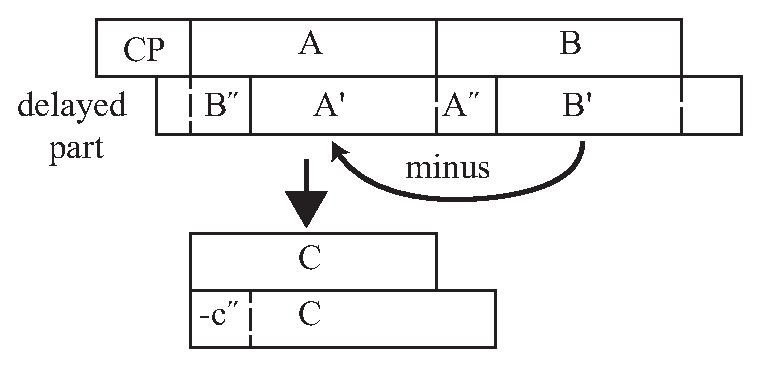
\includegraphics[width=5cm]{effect_of_channel_ACO_OFDM.eps}
		\caption{The illustration for the effect of multipath channels on symbols} \label{fig:effect_of_channel_ACO_OFDM}
	\end{figure}
	Since $C^{'}=A^{'}-B^{'}$ and $C^{''}=A^{''}-B^{''}$, the results of $y(n)-y(n+N/2)$ are shown in Fig.\ref{fig:effect_of_channel_ACO_OFDM}.
	
	If $C$ and $D$ are set to be the ZCC pair sequence and the pair sequence, the aperiodic correlation between $C$ and $D$ is impulse-like.
	%Since there is no frequency offset in VLC systems,
	%As shown in \cite{Qian2017}, the
	Because $ \sum_{n=0}^{N/2-1}C(n+k)D^*(n)=N/2 \delta(k) $, the CSI can be estimated via
	%\begin{small}
	\begin{align}\label{equ:gain_acquire}
        %\begin{split}
          \bar{h}(k)&\nonumber\\
          =&\frac{2}{N}\sum_{n=0}^{N/2-1}(y(n+k)-y(n+k+N/2))D^*(n)\nonumber\\
          =&\frac{2}{N}\sum_{n=0}^{N/2-1}\sum_{l=0}^{L-1}(h(l)(x(n+k-l)-x(n+k-l+N/2))\nonumber\\
          &+w(n+k-l)-w(n+k-l+N/2))D^*(n)\nonumber\\
          =&\frac{2}{N}\sum_{l=0}^{L-1}h(l)\sum_{n=0}^{N/2-1}C(n+k-l)D^*(n)+\tilde{w}(k)\nonumber\\
          =&\sum_{l=0}^{L-1}h(l)\delta(k-l)+\tilde{w}(k).
        %\end{split}
    \end{align}
	%\end{small}
    %where $\tilde{w}(k)$ denotes the noise.

    The next step is to design the required preamble sequence for synchronization and channel estimation. %According to (\ref{equ:sim_transmitter}), all the sub-carriers are needed to generate $ C $. to some extent.

	The detailed steps to generate $ C $ are listed as:

    Step1: Define $S$ as a vector of $N/16+1$ length consisting of $1$ and $-1$:
        $S=[1, \cdots 1, \cdots -1, \ldots -1]^T$.

    Step2: $S$ is multiplied by a matrix $diag([1,j,-1,j^3,\ldots j^{N/16-1},j^{N/16}])$ to be $S_{a}$. This is also called offset quadrature amplitude modulation process.

    Step3: Define $S_b$ as a vector with Hermite property via

        $S_b=[S_{a}(0),S_{a}(1),\cdots S_{a}(N/16),S_{a}^*(N/16-1),\cdots S_{a}^*(1)]^T$.

	Step4: Inverse Fourier transform the $S_b$ to be $S_c$.

    Step5: Finally, we get the required sequence $C$ via $C=[ S_c; S_c; S_c; S_c]\cdot g$. The $g$ is given in \cite{Bellanger2010}.

    According to the relationship of ZCC pair sequences, $D$ is the same as $C$ generated based on PHYDYAS filter. Thus, the preamble in the proposed scheme is designed according to $C$ and the timing offset estimation metric is expressed as
    \begin{eqnarray}\label{equ:synchronization}
          M(k)=\frac{2}{N}\sum_{n=0}^{N/2-1}(y(n+k)-y(n+N/2+k))C^*(n).
    \end{eqnarray}
    Then the timing instant is calculated as
    \begin{equation}\label{equ:d}
            \hat k=\arg\max\limits_{k}(\|M(k)\|),
    \end{equation}
    where $\arg\max\limits_{k}(\|M(k)\|)$ means returning the timing instant $\hat k$ when the absolute value of $M(k)$ is the biggest. It performs an one-dimensional search to find $\hat k$.

    Since the $ h $ is positive, the negative values in $ \bar{h} $ (obtained from (\ref{equ:synchronization}) ) are set to zero to be $ h^{'} $. After the CSI is acquired, the channel frequency response can be calculated via
    \begin{equation}\label{equ:Channel_Fre}
          H(k)=\sum_{l=0}^{L-1}h^{'}e^{-j2\pi\frac{\tau_l k}{N}},0\leq k \leq N-1.
    \end{equation}
    Also, only the odd sub-carriers are transmitting data. Therefore the simplified channel frequency response is expressed as
    \begin{equation}\label{equ:Channel_Fre_sim}
          H(2k+1)=\sum_{l=0}^{L-1}(h^{'}e^{-j2\pi\frac{\tau_l}{N}})e^{-j2\pi\frac{\tau_l k}{N/2}},0\leq k\leq N/2-1.
    \end{equation}
    The calculation complexity of (\ref{equ:Channel_Fre_sim}) is just half of (\ref{equ:Channel_Fre}).

    The received data in frequency domain can be equalized as
    \begin{equation}\label{equ:equalizer}
       X^{'}(2k+1)=\dfrac{2Y(2k+1)}{H(2k+1)},0\leq k\leq N/2-1.
    \end{equation}

    The whole simplified ACO-OFDM system is depict in Fig.\ref{fig:sim_ACO_OFDM_system}.
    \begin{figure}[!htb]
    	\centering 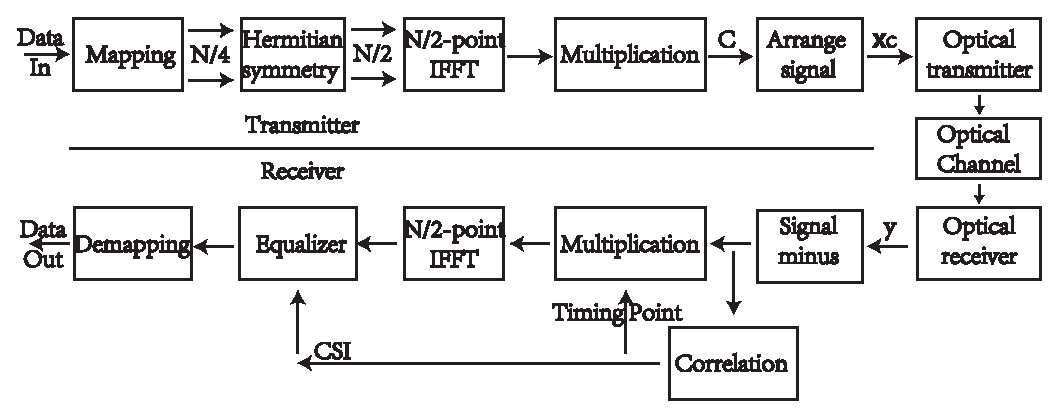
\includegraphics[width=9cm,height=3.5cm]{ACO_OFDM_system.eps}
		\caption{The illustration for the simplified ACO-OFDM system} \label{fig:sim_ACO_OFDM_system}
    \end{figure}
    The IFFT and FFT process in the system are of $ N/2 $ length. After the generation of $ C $, the positive and negative of $ C $ are used to compose ACO-OFDM symbols and the CP is added before transmitted by optical transmitters. The received signals are firstly subtracted. Then results are used to calculate the right timing point via (\ref{equ:synchronization}). When the right timing point is obtained, the needed channel frequency response is calculated via (\ref{equ:Channel_Fre_sim}) after the negative part of synchronization results are set to zero. In the end, data are equalized according to (\ref{equ:equalizer}).



\section{Simulation and Analysis}
	The simulation channel is the indoor manufacturing cell channel given by \cite{Uysal2015Lifi}. Some other simulation parameters are listed in the Table. \ref{Tab:paramters}.

    \begin{table} [htb]
        \caption{The parameters of simulation}
         \centering\begin{tabular}{|l|c|}
                    \hline
                    Parameters & Value\\
                    \hline
                    Number of subcarriers & 512 \\
                    \hline
                    CP length & 64\\
                    \hline
                    Frame length & 16 OFDM symbols\\
                    \hline
                    Bandwidth & 500MHz \\
                    \hline
                    Constellation order & 16QAM \\
                    %Maximum time delay $\tau_{max}$ & 50  \\
                    %Number of paths L & [$0.1\tau_{max}$,$0.9\tau_{max}$] \\
                    %Pilot distribution & Scattered \\
                    \hline
                    Simulation trial number & 100000 \\
                    \hline
                    Room area W$\times$H$\times$L & 2$\times$4$\times$3$m^3$\\
                    \hline
                    Receiving node(PD)area & 1$cm^2$ \\
                    \hline
                    Conversion efficient of photoelectricity & $0.5A/W$ \\
                    \hline
                    Receiver field of view(FOV) & $60^{\circ}$ \\
                    \hline
                    \end{tabular}
         \label{Tab:paramters}
    \end{table}


	\begin{figure}[!htb]
    	\centering 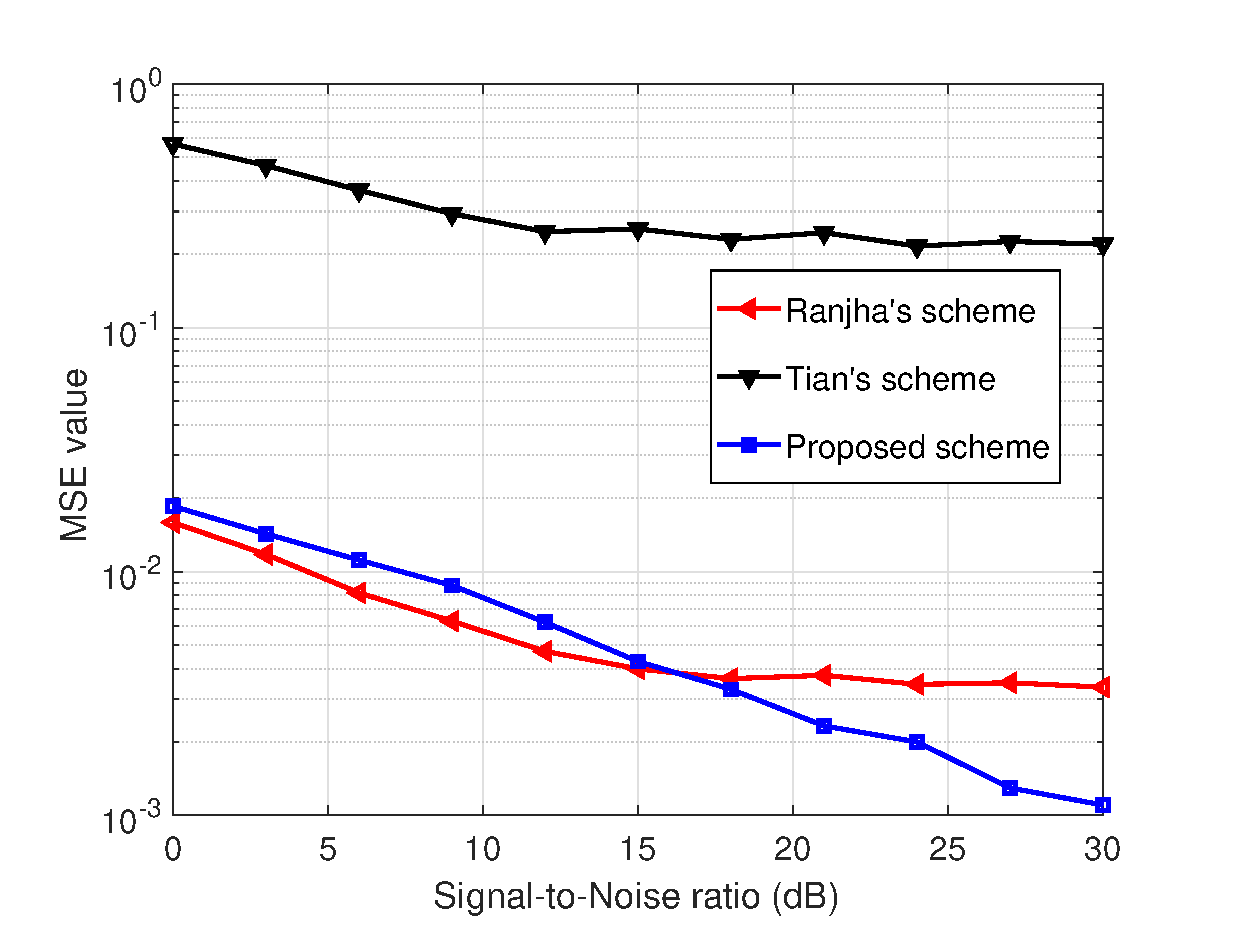
\includegraphics[width=7cm]{synchronization_mse.eps}
		\caption{The MSE performance comparison of synchronization schemes} \label{fig:synchronization_mse}
    \end{figure}
    Fig.\ref{fig:synchronization_mse} shows the normalized MSE value of timing offset estimation with respect to the IFFT length. The MSE values of the three schemes decrease with enlarging the SNR value. The Tian's scheme achieves the worst performance compared with the Ranjha's and proposed schemes. When SNR value is large, the estimation error is just one third of that of Ranjha's scheme. If the SNR is below 16 dB, the Ranjha's scheme has better performance but the performance difference is small.
    %As to the calculation complexity, the Tian's scheme needs $ N/2-2 $ multiplications at each discrete sample time, while Bilal's \cite{Ranjha2015} and proposed schemes both need
    In \cite{chow2013adaptive}, the OFDM-based VLC systems using common LEDs are tested and the suggested SNR values are over 18dB.
    Thus, the proposed scheme is good enough.

    \begin{figure}[!htb]
    	\centering 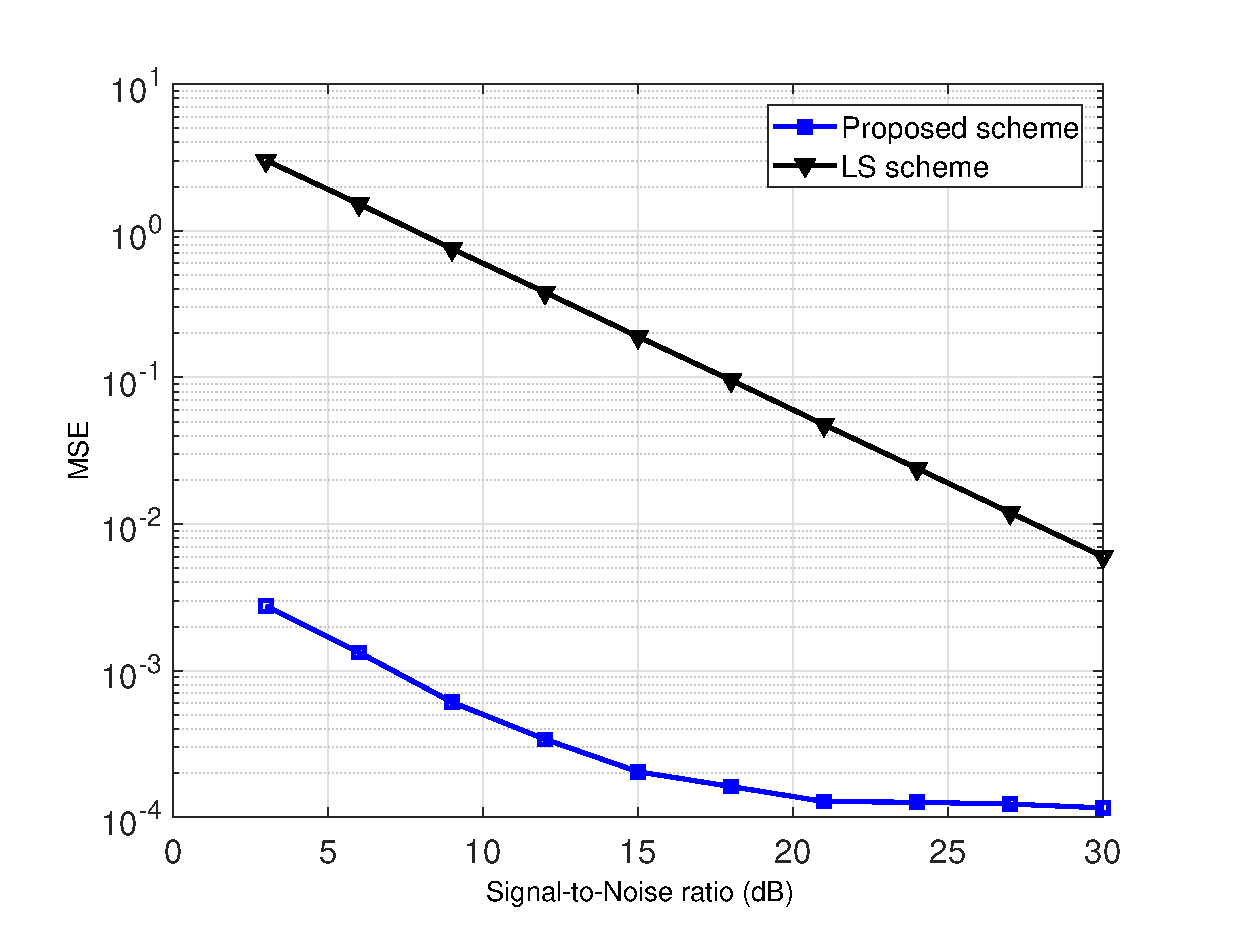
\includegraphics[width=7cm]{channel_estimation_HMSE.eps}
		\caption{The channel frequency estimation performance comparison of LS and proposed scheme}
        \label{fig:channel_estimation_HMSE}
    \end{figure}
    Fig.\ref{fig:channel_estimation_HMSE} presents a comparison of channel frequency response estimation performance. The channel frequency estimation MSE value of LS scheme decreases with enlarging SNR with steady slope, while the MSE value of proposed scheme drops gradually to a level but is much lower than that of LS scheme. The proposed scheme has better channel estimation performance than LS scheme.

    %In terms of the calculation complexity, for the proposed algorithm, most calculation can be done via the system FFT module. Only $ N/2 $ multiplications are needed for the simplified channel frequency response.
    %The proposed algorithm is easier than conventional

    \begin{figure}[!htb]
    	\centering 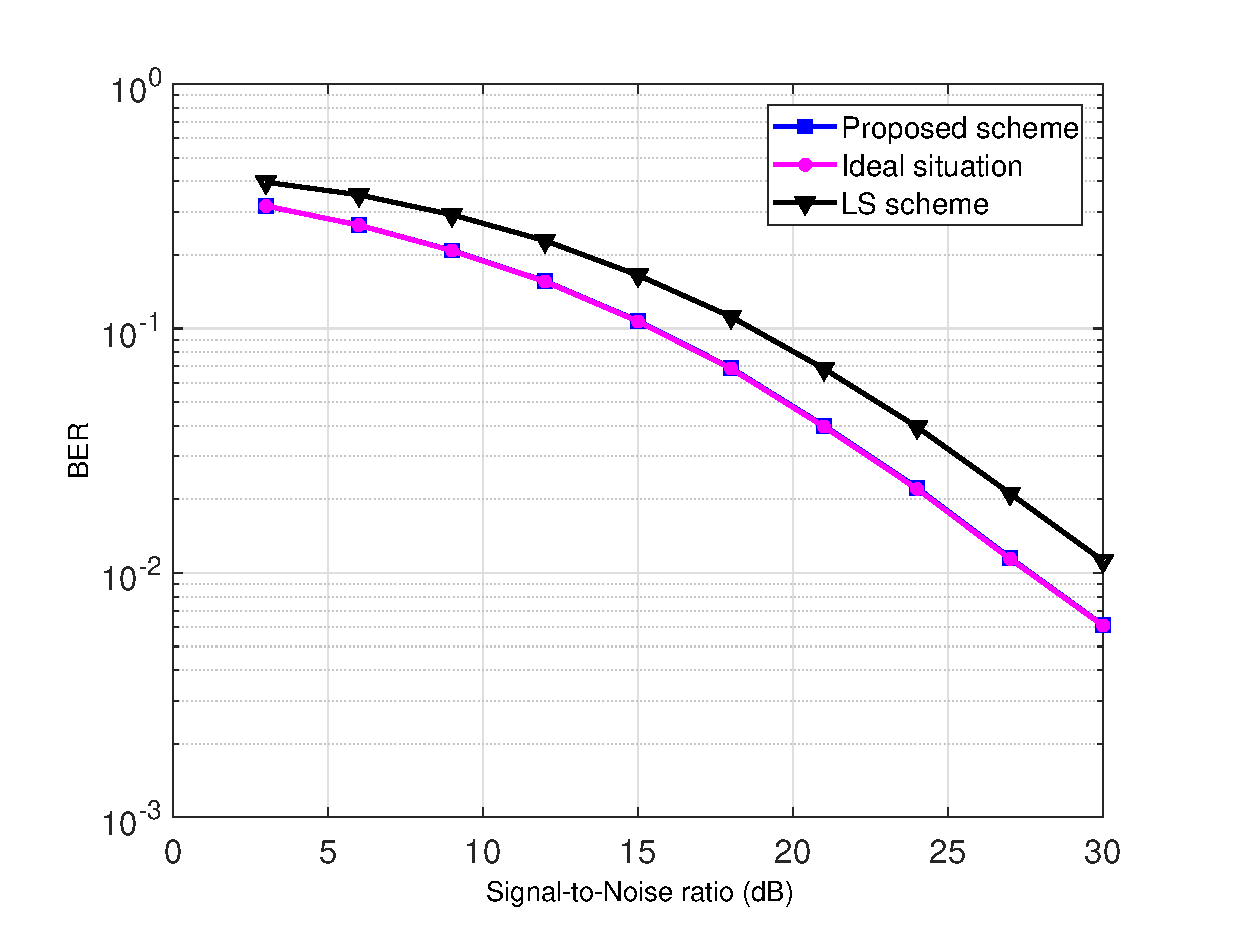
\includegraphics[width=7cm]{channel_estimation_BER.eps}
		\caption{The BER performance comparison of LS and proposed scheme} \label{fig:channel_estimation_BER}
    \end{figure}

	Fig.\ref{fig:channel_estimation_BER} shows BER performances of the LS scheme, proposed scheme and the ideal performance with prior knowledge of CSI. The proposed scheme has BER performance similar to the ideal performance and is better than LS scheme.
	
	%Overall, the proposed joint synchronization and channel estimation scheme has better performance than other schemes.

\section{Conclusion}
In this letter, a joint synchronization and channel estimation scheme is proposed for ACO-OFDM systems. A simplified transceiver is proposed which only needs half the calculations compared with conventional transceiver. Simulations have revealed that the proposed scheme has better timing MSE performance than Tian's and Ranjha's schemes in synchronization task and has better channel frequency response MSE performance and BER performance than LS channel estimation scheme.


\scriptsize{\bibliography{mybibtex}}
\end{document}
